\section{Clasificación de grupos abelianos finitos}

\begin{ejercicio}\label{ej:7.1}
    Calcular los órdenes de todos los elementos de los distintos grupos abelianos de orden $8$, $12$, $16$ y $24$.
    \begin{enumerate}
        \item Sea $G$ un grupo abeliano de $|G| = 8$.
        
        Como $|G|=8=2^3$, por la estructura de los grupos abelianos finitos, tenemos que hay tres posibilidades:
        \begin{enumerate}
            \item $G \cong C_8$.
            
            Como el orden se mantiene bajo isomorfismos, basta con encontrar el orden de los elementos del grupo cíclico $C_8\cong \bb{Z}_8$.
            \begin{equation*}
                O(x) = \frac{8}{\mcd(x, 8)}.
            \end{equation*}

            Por tanto, los órdenes de los elementos de $C_8$ son:
            \begin{equation*}
                O(0) = 1, \quad
                O(1) = O(3) = O(5) = O(7) = 8, \quad
                O(2) = O(6) = 4, \quad
                O(4) = 2.
            \end{equation*}

            Por tanto, hay un elemento de orden $1$, cuatro de orden $8$, dos de orden $4$ y uno de orden $2$.

            \item $G \cong C_4 \oplus C_2$.
            \begin{equation*}
                O(x, y) = \mcm(O(x), O(y))\qquad \forall x \in C_4, y \in C_2.
            \end{equation*}

            Los órdenes de $\bb{Z}_2$ son:
            \begin{equation*}
                O(0) = 1, \quad O(1) = 2.
            \end{equation*}

            Los órdenes de $\bb{Z}_4$ son:
            \begin{equation*}
                O(0) = 1, \quad O(1) = O(3) = 4, \quad O(2) = 2.
            \end{equation*}

            Por tanto, los órdenes de los elementos de $C_4 \oplus C_2$ son:
            \begin{gather*}
                O(0, 0) = 1, \quad
                O(1, 0) = O(1,1) = O(3, 0) = O(3, 1) = 4, \\
                O(2, 0) = O(2, 1) = 2, \quad
                O(0, 1) = 2.
            \end{gather*}
            Por tanto, hay un elemento de orden $1$, cuatro de orden $4$ y tres de orden~$2$.
            \item $G \cong C_2 \oplus C_2 \oplus C_2$.
            
            Los órdenes de $\bb{Z}_2$ son:
            \begin{equation*}
                O(0) = 1, \quad O(1) = 2.
            \end{equation*}
            Por tanto, los órdenes de los elementos de $C_2 \oplus C_2 \oplus C_2$ son:
            \begin{align*}
                O(0, 0, 0) &= 1, \\
                O(x,y,z) &= 2 \qquad \forall x,y,z \in \{0,1\} \text{ tal que } x+y+z \neq 0.
            \end{align*}
            Por tanto, hay un elemento de orden $1$ y siete de orden $2$.
        \end{enumerate}



        \item Sea $G$ un grupo abeliano de $|G| = 12$.
        
        Como $|G|=12=2^2 \cdot 3$, por la estructura de los grupos abelianos finitos, tenemos que hay varias posibilidades:
        \begin{enumerate}
            \item $G \cong C_{12}$.
            
            Como el orden se mantiene bajo isomorfismos, basta con encontrar el orden de los elementos del grupo cíclico $C_{12}\cong \bb{Z}_{12}$.
            \begin{equation*}
                O(x) = \frac{12}{\mcd(x, 12)}.
            \end{equation*}

            Por tanto, los órdenes de los elementos de $C_{12}$ son:
            \begin{gather*}
                O(0) = 1, \quad
                O(1) = O(5) = O(7) = O(11) = 12, \quad
                O(2) = O(10) = 6,\\
                O(3) = O(9) = 4, \quad
                O(4) = O(8) = 3, \quad
                O(6) = 2.
            \end{gather*}

            
            \item $G \cong C_6 \oplus C_2$.
            
            Como el orden se mantiene bajo isomorfismos, basta con encontrar el orden de los elementos del grupo cíclico $C_6\cong \bb{Z}_6$ y de $C_2\cong \bb{Z}_2$.
            Los órdenes de $\bb{Z}_2$ son:
            \begin{equation*}
                O(0) = 1, \quad O(1) = 2.
            \end{equation*}
            Los órdenes de $\bb{Z}_6$ son:
            \begin{equation*}
                O(0) = 1, \quad O(1) = O(5) = 6, \quad O(2) = O(4) = 3, \quad O(3) = 2.
            \end{equation*}

            Por tanto, los órdenes de los elementos de $C_6 \oplus C_2$ son:
            \begin{gather*}
                O(0, 0) = 1, \\
                O(1, 0) = O(5, 0) = O(1, 1) = O(5, 1) = 6, \\
                O(2, 0) = O(4, 0) = 3, \\
                O(2, 1) = O(4, 1) = 6, \\
                O(3, 0) = O(3, 1) = 2, \\
                O(0, 1) = 2.
            \end{gather*}
            
        \end{enumerate}


        \item Sea $G$ un grupo abeliano de $|G| = 16$.
        
        Como $|G|=16=2^4$, por la estructura de los grupos abelianos finitos, tenemos que hay varias posibilidades:
        \begin{enumerate}
            \item $G \cong C_{16}$.
            
            Como el orden se mantiene bajo isomorfismos, basta con encontrar el orden de los elementos del grupo cíclico $C_{16}\cong \bb{Z}_{16}$.
            \begin{equation*}
                O(x) = \frac{16}{\mcd(x, 16)}.
            \end{equation*}
            Por tanto, los órdenes de los elementos de $C_{16}$ son:
            \begin{gather*}
                O(0) = 1, \\
                O(1) = O(3) = O(5) = O(7) = O(9) = O(11) = O(13) = O(15) = 16, \\
                O(2) = O(6) = O(10) = O(14) = 8, \\
                O(4) = O(12) = 4.
            \end{gather*}
            
            \item $G \cong C_8 \oplus C_2$.
            
            Como el orden se mantiene bajo isomorfismos, basta con encontrar el orden de los elementos del grupo cíclico $C_8\cong \bb{Z}_8$ y de $C_2\cong \bb{Z}_2$.
            Los órdenes de $\bb{Z}_2$ son:
            \begin{equation*}
                O(0) = 1, \quad O(1) = 2.
            \end{equation*}

            Los órdenes de $\bb{Z}_8$ los hemos calculado en el primer apartado:
            \begin{equation*}
                O(0) = 1, \quad
                O(1) = O(3) = O(5) = O(7) = 8, \quad
                O(2) = O(6) = 4, \quad
                O(4) = 2.
            \end{equation*}

            Por tanto, los órdenes de los elementos de $C_8 \oplus C_2$ son:
            \begin{gather*}
                O(0, 0) = 1, \qquad O(0,1)= 2, \\
                O(1, 0) = O(3, 0) = O(5, 0) = O(7, 0) = 8, \\
                O(1, 1) = O(3, 1) = O(5, 1) = O(7, 1) = 8, \\
                O(2, 0) = O(6, 0) = O(2, 1) = O(6, 1) = 4, \\
                O(4, 0) = O(4, 1) = 2.
            \end{gather*}

            \item $G \cong C_4 \oplus C_4$.
            
            Como el orden se mantiene bajo isomorfismos, basta con encontrar el orden de los elementos del grupo cíclico $C_4\cong \bb{Z}_4$.
            Los órdenes de $\bb{Z}_4$ son:
            \begin{equation*}
                O(0) = 1, \quad O(1) = O(3) = 4, \quad O(2) = 2.
            \end{equation*}
            Por tanto, los órdenes de los elementos de $C_4 \oplus C_4$ son:
            \begin{gather*}
                O(0, 0) = 1\\
                O(0,1) = O(0,3) = O(1,1) = O(1,3) = O(2,1) = O(2,3) = O(3,1) = O(3,3) = 4, \\
                O(1,0) = O(1,2) = O(3,0) = O(3,2) = 4, \\
                O(0,2) = O(2,0) = O(2,2) = 2
            \end{gather*}
            \item $G \cong C_4 \oplus C_2 \oplus C_2$.
            
            Como el orden se mantiene bajo isomorfismos, basta con encontrar el orden de los elementos del grupo $C_4\oplus C_2 \oplus C_2$. Los órdenes de $C_4\oplus C_2$ ya los hemos calculado anteriormente:
            \begin{gather*}
                O(0, 0) = 1, \\
                O(1, 0) = O(1,1) = O(3, 0) = O(3, 1) = 4, \\
                O(2, 0) = O(2, 1) = 2, \\
                O(0, 1) = 2.
            \end{gather*}

            Los órdenes de $C_2$ son:
            \begin{equation*}
                O(0) = 1, \quad O(1) = 2.
            \end{equation*}

            Por tanto, los órdenes de los elementos de $C_4 \oplus C_2 \oplus C_2$ son:
            \begin{gather*}
                O(0, 0, 0) = 1, \\
                O(1, 0, 0) = O(1, 1, 0) = O(3, 0, 0) = O(3, 1, 0) = 4, \\
                O(2, 0, 0) = O(2, 1, 0) = 2, \\
                O(0, 1, 0) = 2, \\
                O(0, 0, 1) = 2, \\
                O(1, 0, 1) = O(1, 1, 1) = O(3, 0, 1) = O(3, 1, 1) = 4, \\
                O(2, 0, 1) = O(2, 1, 1) = 2, \\
                O(0, 1, 1) = 2.
            \end{gather*}
            
            \item $G \cong C_2 \oplus C_2 \oplus C_2 \oplus C_2$.
            
            Como el orden se mantiene bajo isomorfismos, basta con encontrar el orden de los elementos del grupo $C_2\oplus C_2 \oplus C_2 \oplus C_2$. Los órdenes de $C_2\oplus C_2 \oplus C_2$ ya los hemos calculado anteriormente:
            \begin{align*}
                O(0, 0, 0) &= 1, \\
                O(x, y, z) &= 2 \qquad \forall x,y,z \in \{0,1\} \text{ tal que } x+y+z \neq 0.
            \end{align*}

            Por tanto, los órdenes de los elementos de $C_2 \oplus C_2 \oplus C_2 \oplus C_2$ son:
            \begin{align*}
                O(0, 0, 0, 0) &= 1, \\
                O(x, y, z, w) &= 2 \qquad \forall x,y,z,w \in \{0,1\} \text{ tal que } x+y+z+w \neq 0.
            \end{align*}
        \end{enumerate}

        \item Sea $G$ un grupo abeliano de $|G| = 24$.
        
        Como $|G|=24=2^3 \cdot 3$, por la estructura de los grupos abelianos finitos, tenemos que hay varias posibilidades:
        \begin{enumerate}
            \item $G \cong C_{24}$.
            
            Como el orden se mantiene bajo isomorfismos, basta con encontrar el orden de los elementos del grupo cíclico $C_{24}\cong \bb{Z}_{24}$.
            \begin{equation*}
                O(x) = \frac{24}{\mcd(x, 24)}.
            \end{equation*}

            Por tanto, los órdenes de los elementos de $C_{24}$ son:
            \begin{gather*}
                O(0) = 1, \\
                O(1) = O(5) = O(7) = O(11) = O(13) = O(17) = O(19) = O(23) = 24, \\
                O(2) = O(10) = O(14) = O(22) = 12, \\
                O(3) = O(9) = O(15) = 8, \\
                O(4) = O(20) = 6, \\
                O(6) = O(18) = 4, \\
                O(8) = O(16) = 3, \\
                O(12) = 2.
            \end{gather*}
            
            \item $G \cong C_{12} \oplus C_2$.
            
            Como el orden se mantiene bajo isomorfismos, basta con encontrar el orden de los elementos del grupo cíclico $C_{12}\cong \bb{Z}_{12}$ y de $C_2\cong \bb{Z}_2$.
            Los órdenes de $\bb{Z}_12$ los hemos calculado anteriormente:
            \begin{gather*}
                O(0) = 1, \\
                O(1) = O(5) = O(7) = O(11) = 12, \\
                O(2) = O(10) = 6, \\
                O(3) = O(9) = 4, \\
                O(4) = O(8) = 3, \\
                O(6) = 2.
            \end{gather*}

            Los órdenes de $\bb{Z}_2$ son:
            \begin{equation*}
                O(0) = 1, \quad O(1) = 2.
            \end{equation*}

            Por tanto, los órdenes de los elementos de $C_{12} \oplus C_2$ son:
            \begin{gather*}
                O(0, 0) = 1, \\
                O(1, 0) = O(5, 0) = O(7, 0) = O(11, 0) = 12, \\
                O(2, 0) = O(10, 0) = 6, \\
                O(3, 0) = O(9, 0) = 4, \\
                O(4, 0) = O(8, 0) = 3, \\
                O(6, 0) = 2, \\
                O(0, 1) = 2, \\
                O(1, 1) = O(5, 1) = O(7, 1) = O(11, 1) = 12, \\
                O(2, 1) = O(10, 1) = 6, \\
                O(3, 1) = O(9, 1) = 4, \\
                O(4, 1) = O(8, 1) = 6, \\
                O(6, 1) = 2.
            \end{gather*}
            
            \item $G \cong C_6 \oplus C_2 \oplus C_2$.
            
            Como el orden se mantiene bajo isomorfismos, basta con encontrar el orden de los elementos del grupo $C_6\oplus C_2 \oplus C_2$. Los órdenes de $C_6\oplus C_2$ ya los hemos calculado anteriormente:
            \begin{gather*}
                O(0, 0) = 1, \\
                O(1, 0) = O(5, 0) = O(1, 1) = O(5, 1) = 6, \\
                O(2, 0) = O(4, 0) = 3, \\
                O(2, 1) = O(4, 1) = 6, \\
                O(3, 0) = O(3, 1) = 2, \\
                O(0, 1) = 2.
            \end{gather*}

            Los órdenes de $C_2$ son:
            \begin{equation*}
                O(0) = 1, \quad O(1) = 2.
            \end{equation*}

            Por tanto, los órdenes de los elementos de $C_6 \oplus C_2 \oplus C_2$ son:
            \begin{gather*}
                O(0, 0, 0) = 1, \\
                O(1, 0, 0) = O(5, 0, 0) = O(1, 1, 0) = O(5, 1, 0) = 6, \\
                O(2, 0, 0) = O(4, 0, 0) = 3, \\
                O(2, 1, 0) = O(4, 1, 0) = 6, \\
                O(3, 0, 0) = O(3, 1, 0) = 2, \\
                O(0, 1, 0) = 2, \\
                O(0, 0, 1) = 2, \\
                O(1, 0, 1) = O(5, 0, 1) = O(1, 1, 1) = O(5, 1, 1) = 6, \\
                O(2, 0, 1) = O(4, 0, 1) = O(2, 1, 1) = O(4, 1, 1) = 6, \\
                O(3, 0, 1) = O(3, 1, 1) = 2, \\
                O(0, 1, 1) = 2.
            \end{gather*}
        \end{enumerate}







    \end{enumerate}
\end{ejercicio}

\begin{ejercicio}\label{ej:7.2}
    Para los siguientes grupos calcular sus descomposiciones cíclicas.
    \begin{enumerate}
        \item $G_1 = \{1, 8, 12, 14, 18, 21, 27, 31, 34, 38, 44, 47, 51, 53, 57, 64\}$ con operación dada por multiplicación módulo $65$.\\
        
        Vemos que $G_1$ es un abeliano con $|G_1| = 16$. Entonces, por el Ejercicio~\ref{ej:7.1}, sabemos que $G_1$ es isomorfo a uno de los siguientes grupos:
        \begin{enumerate}
            \item $C_{16}$.
            \item $C_8 \oplus C_2$.
            \item $C_4 \oplus C_4$.
            \item $C_4 \oplus C_2 \oplus C_2$.
            \item $C_2 \oplus C_2 \oplus C_2 \oplus C_2$.
        \end{enumerate}

        Para distinguir, calculamos los órdenes de los elementos de $G_1$:
        \begin{gather*}
            O(1) = 1, \\
            O(8) = O(12) = O(18) = O(21) = O(27) = O(31) = O(34) = 4\\
            O(38) = O(44) = O(47) = O(53) = O(57) = 4, \\
            O(14) = O(51) = O(64) = 2.
        \end{gather*}

        Por tanto, la única posibilidad es que $G_1 \cong C_4 \oplus C_4$.
        \item $G_2 = \{1, 8, 17, 19, 26, 28, 37, 44, 46, 53, 62, 64, 71, 73, 82, 89, 91, 98, 107,109, 116, 118, 127, 134\}$ con operación dada por multiplicación módulo $135$.
        
        Vemos que $G_2$ es un abeliano con $|G_2| = 24$. Entonces, por el Ejercicio~\ref{ej:7.1}, sabemos que $G_2$ es isomorfo a uno de los siguientes grupos:
        \begin{enumerate}
            \item $C_{24}$.
            \item $C_{12} \oplus C_2$.
            \item $C_6 \oplus C_2 \oplus C_2$.
        \end{enumerate}

        Para distinguir, calculamos los órdenes de los elementos de $G_2$ (es tedioso, pero sencillo. En nuestro caso, lo hemos implementado mediante un sencillo programa). Nos bastaría con calcular:
        \begin{gather*}
            O(28)=O(53)=O(82)=O(107)=4
        \end{gather*}
        Por tanto, la única posibilidad es que:
        \begin{equation*}
            G_2 \cong C_6 \oplus C_2 \oplus C_2.
        \end{equation*}
        \item $G_3 = \{1, 7, 17, 23, 49, 55, 65, 71\}$ con operación dada por multiplicación módulo $96$.
        
        Vemos que $G_3$ es un abeliano con $|G_3| = 8$. Entonces, por el Ejercicio~\ref{ej:7.1}, sabemos que $G_3$ es isomorfo a uno de los siguientes grupos:
        \begin{enumerate}
            \item $C_8$.
            \item $C_4 \oplus C_2$.
            \item $C_2 \oplus C_2 \oplus C_2$.
        \end{enumerate}

        Para distinguir, calculamos los órdenes de los elementos de $G_3$. De nuevo, es tedioso, pero sencillo. Basta con calcular:
        \begin{equation*}
            O(17) = O(49) = O(65) = 2\qquad O(7)=4
        \end{equation*}

        Por tanto, la única posibilidad es que:
        \begin{equation*}
            G_3 \cong C_4 \oplus C_2.
        \end{equation*}
        \item $G_4 = \{1, 4, 11, 14, 16, 19, 26, 29, 31, 34, 41, 44\}$ con operación dada por multiplicación módulo $45$.
        
        Vemos que $G_4$ es un abeliano con $|G_4| = 12$. Entonces, por el Ejercicio~\ref{ej:7.1}, sabemos que $G_4$ es isomorfo a uno de los siguientes grupos:
        \begin{enumerate}
            \item $C_{12}$.
            \item $C_6 \oplus C_2$.
        \end{enumerate}
        Para distinguir, calculamos los órdenes de los elementos de $G_4$. De nuevo, es tedioso, pero sencillo. Basta con calcular:
        \begin{gather*}
            O(19)=O(26)=O(44)=2
        \end{gather*}

        Por tanto, la única posibilidad es que:
        \begin{equation*}
            G_4 \cong C_6 \oplus C_2.
        \end{equation*}
    \end{enumerate}
\end{ejercicio}

\begin{ejercicio}\label{ej:7.3}
    Calcular la descomposición cíclica y cíclica primaria de los grupos abelianos $C_{24} \oplus C_{40} \oplus C_{35}$ y $C_{14} \oplus C_{100} \oplus C_{40}$. ¿Son isomorfos?\\

    Tenemos que:
    \begin{align*}
        24&=2^3 \cdot 3, \\
        40&=2^3 \cdot 5, \\
        35&=5 \cdot 7, \\
        14&=2 \cdot 7, \\
        100&=2^2 \cdot 5^2, \\
        40&=2^3 \cdot 5.
    \end{align*}

    Por tanto, vemos a simple vista sin necesidad de hacer cálculos que no tienen el mismo orden, luego no son isomorfos.
    Trabajamos ahora con cada uno por separado.
    \begin{enumerate}
        \item Para $C_{24} \oplus C_{40} \oplus C_{35}$:
        
        Tenemos que:
        \begin{align*}
            C_{24} \oplus C_{40} \oplus C_{35} &\cong C_{2^3} \oplus C_3 \oplus C_{2^3} \oplus C_5 \oplus C_{5} \oplus C_7 \\
            &\cong C_{2^3} \oplus C_{2^3} \oplus C_3 \oplus C_5 \oplus C_5 \oplus C_7
        \end{align*}

        Por tanto, esa es la descomposición cíclica primaria:
        \begin{equation*}
            C_{24} \oplus C_{40} \oplus C_{35} \cong C_{2^3} \oplus C_{2^3} \oplus C_3 \oplus C_5 \oplus C_5 \oplus C_7.
        \end{equation*}

        En vistas de calcular la descomposición cíclica, tenemos la siguiente matriz:
        \begin{equation*}
            \begin{pmatrix}
                2^3 & 2^3\\
                3 & 1\\
                5 & 5\\
                7 & 1
            \end{pmatrix}
            \Longrightarrow
            \left\{
                \begin{array}{l}
                    d_1 = 2^3\cdot 3\cdot 5\cdot 7 = 840, \\
                    d_2 = 2^3\cdot 5 = 40
                \end{array}
            \right.
        \end{equation*}

        Por tanto, la descomposición cíclica es:
        \begin{equation*}
            C_{24} \oplus C_{40} \oplus C_{35} \cong C_{840} \oplus C_{40}.
        \end{equation*}

        \item Para $C_{14} \oplus C_{100} \oplus C_{40}$:
        
        Tenemos que:
        \begin{align*}
            C_{14} \oplus C_{100} \oplus C_{40} &\cong C_{2} \oplus C_7 \oplus C_{2^2} \oplus C_{5^2} \oplus C_{2^3} \oplus C_5 \\
            &\cong C_{2^3}\oplus C_{2^2} \oplus C_2 \oplus C_{5^2} \oplus C_5 \oplus C_7
        \end{align*}
        Por tanto, esa es la descomposición cíclica primaria:
        \begin{equation*}
            C_{14} \oplus C_{100} \oplus C_{40} \cong C_{2^3}\oplus C_{2^2} \oplus C_2 \oplus C_{5^2} \oplus C_5 \oplus C_7.
        \end{equation*}
        En vistas de calcular la descomposición cíclica, tenemos la siguiente matriz:
        \begin{equation*}
            \begin{pmatrix}
                2^3 & 2^2 & 2\\
                5^2 & 5 & 1\\
                7 & 1 & 1
            \end{pmatrix}
            \Longrightarrow
            \left\{
                \begin{array}{l}
                    d_1 = 2^3\cdot 5^2\cdot \cdot 7 = 1400, \\
                    d_2 = 2^2\cdot 5 = 20, \\
                    d_3 = 2
                \end{array}
            \right.
        \end{equation*}

        Por tanto, la descomposición cíclica es:
        \begin{equation*}
            C_{14} \oplus C_{100} \oplus C_{40} \cong C_{1400} \oplus C_{20} \oplus C_2.
        \end{equation*}
    \end{enumerate}

    Como vemos, las descomposiciones cíclicas son diferentes, lo que también nos indica que los grupos no son isomorfos.
\end{ejercicio}

\begin{ejercicio}\label{ej:7.4}
    Sea $G$ el grupo de las simetrías de un rectángulo (no cuadrado). Probar que $G$ es un grupo abeliano. Calcular sus descomposiciones cíclica y cíclica primaria.\\


    Las simetrías de un rectángulo se muestran en la Figura~\ref{fig:simetria_rectangulo}.
    \begin{figure}[h]
        \centering
        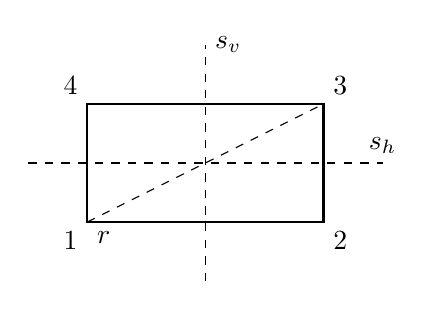
\begin{tikzpicture}[scale=1.5]
            \draw[thick] (0,0) rectangle (2,1);
            
            % Notamos los 4 vértices
            \node at (0,0) [below left] {$1$};
            \node at (2,0) [below right] {$2$};
            \node at (2,1) [above right] {$3$};
            \node at (0,1) [above left] {$4$};

            % Rotación de 180 grados. Diagonal desde 1 a 3
            \draw[dashed] (0,0) -- (2,1) node [pos=0, below right] {$r$};

            % Simetrias eje vertical y horizontal
            \draw[dashed] (1,-0.5) -- (1,1.5) node [pos=1, right] {$s_v$};
            \draw[dashed] (-0.5,0.5) -- (2.5,0.5) node [pos=1, above] {$s_h$};
        \end{tikzpicture}
        \caption{Simetrías de un rectángulo.}
        \label{fig:simetria_rectangulo}
    \end{figure}
    Para ver que se trata de un grupo, damos su tabla de Cayley:
    \begin{equation*}
        \begin{tabular}{c|cccc}
            $\cdot$ & $e$ & $r$ & $s_v$ & $s_h$ \\
            \hline
            $e$ & $e$ & $r$ & $s_v$ & $s_h$ \\
            $r$ & $r$ & $e$ & $s_h$ & $s_v$ \\
            $s_v$ & $s_v$ & $s_h$ & $e$ & $r$ \\
            $s_h$ & $s_h$ & $s_v$ & $r$ & $e$
        \end{tabular}
    \end{equation*}

    Como vemos, $G$ es un grupo. Además, es abeliano porque la tabla es simétrica respecto a la diagonal principal. Como $|G|=4$, hay dos opciones:
    \begin{enumerate}
        \item $G \cong C_4$.
        \item $G \cong C_2 \oplus C_2$.
    \end{enumerate}

    Como $G$ no es cíclico (pues todos los elementos tienen orden $2$), tenemos que:
    \begin{equation*}
        G \cong C_2 \oplus C_2.
    \end{equation*}

    Esta es tanto su descomposición cíclica como cíclica primaria.
\end{ejercicio}

\begin{ejercicio}\label{ej:7.5}
    Sea $G$ un grupo abeliano de orden $n$ y $l(G)$ su longitud. Si la descomposición de $n$ en factores primos es $n = p_1^{e_1} \cdots p_r^{e_r}$, demostrar que
    \begin{equation*}
        l(G) = e_1 + \cdots + e_r,
    \end{equation*}
    y que
    \begin{equation*}
        \fact(G) = (C_{p_1},\stackrel{(e_1)}{\ldots}, C_{p_1}, \ldots, C_{p_r},\stackrel{(e_r)}{\ldots}, C_{p_r}).
    \end{equation*}
    En particular, todos los grupos abelianos del mismo orden tienen la misma longitud y la misma lista de factores de composición.\\

    Como $G$ es abeliano, es resoluble y el enunciado tiene sentido. Calculamos su descomposición cíclica primaria, de forma que $\exists t_1,t_2,\dots,t_r\in \bb{N}$ de forma que, para el $i-$ésimo entero $t_i$ existe una partición de $e_i$ en $t_i$ sumandos:
    \begin{gather*}
        n_{i1} \geq n_{i2} \geq \cdots \geq n_{it_i} \geq 1, \\
        e_i = n_{i1} + n_{i2} + \cdots + n_{it_i}.
    \end{gather*}

    De esta forma, tenemos que:
    \begin{equation*}
        G \cong \bigoplus_{i=1}^r \bigoplus_{j=1}^{t_i} C_{p_i^{n_{ij}}}.
    \end{equation*}

    Por el Ejercicio~\ref{ej:5.7}, tenemos que:
    \begin{align*}
        l(G) &= \sum_{i=1}^r \sum_{j=1}^{t_i} n_{ij} \AstIg \sum_{i=1}^r e_i = e_1 + \cdots + e_r\\
        \fact(G) &= \bigcup_{i=1}^r \bigcup_{j=1}^{t_i} \fact(C_{p_i^{n_{ij}}})
    \end{align*}
    donde en $(\ast)$ hemos empleado que es una partición y, por tanto, suman $e_i$.\\

    Por el Ejercicio~\ref{ej:5.8}, como $C_{p_i^{n_{ij}}}$ es cíclico, tenemos que:
    \begin{equation*}
        \fact(C_{p_i^{n_{ij}}}) = (C_{p_i},\stackrel{(n_{ij})}{\ldots}, C_{p_i})\qquad \forall i,j.
    \end{equation*}

    Por tanto, tenemos que:
    \begin{align*}
        \fact(G) &= \bigcup_{i=1}^r \bigcup_{j=1}^{t_i} (C_{p_i},\stackrel{(n_{ij})}{\ldots}, C_{p_i}) \AstIg \bigcup_{i=1}^r (C_{p_i},\stackrel{(e_i)}{\ldots}, C_{p_i})
        = (C_{p_1},\stackrel{(e_1)}{\ldots}, C_{p_1}, \ldots, C_{p_r},\stackrel{(e_r)}{\ldots}, C_{p_r}).
    \end{align*}
    donde, de nuevo, en $(\ast)$ hemos empleado que es una partición y, por tanto, suman $e_i$. Hemos demostrado por tanto lo pedido.
\end{ejercicio}

\begin{ejercicio}\label{ej:7.6}
    Listar todos los grupos abelianos no isomorfos de orden $10$, $16$, $20$, $30$, $40$, $108$ y $360$, dando sus factores invariantes, divisores elementales y descomposiciones cíclicas y cíclicas primarias.
    % // TODO: Hacer
\end{ejercicio}

\begin{ejercicio}\label{ej:7.7}
    Calcular la forma normal, los factores invariantes y los divisores elementales de las siguientes matrices:
    \begin{align*}
        &A_1 = \begin{pmatrix}
            0 & 2 & 0 \\
            -6 & -4 & -6 \\
            6 & 6 & 6 \\
            7 & 10 & 6
        \end{pmatrix},
        &A_2 = \begin{pmatrix}
            -22 & -48 & -267 \\
            -4 & -4 & 31 \\
            -4 & -24 & 105 \\
            4 & -6 & -6
        \end{pmatrix},\\
        &A_3 = \begin{pmatrix}
            9 & 4 & 5 \\
            -4 & 0 & -3 \\
            -6 & -4 & -2
        \end{pmatrix},
        &A_4 = \begin{pmatrix}
            4 & 0 & 0 \\
            0 & 6 & 0 \\
            0 & 0 & 8
        \end{pmatrix}.
    \end{align*}
\end{ejercicio}

\begin{ejercicio}\label{ej:7.8}
    Para los siguientes grupos abelianos calcular sus rangos y sus descomposiciones cíclicas y cíclicas primarias. ¿Son algunos de estos grupos isomorfos?
    \begin{enumerate}
        \item $G_1 = \left\langle a, b, c \left|
            \begin{array}{rcl}
                3a + 9b + 9c &=& 0 \\
                9a - 3b + 9c &=& 0
            \end{array}
        \right.\right\rangle$.
        \item $G_2 = \left\langle a, b, c \left|
            \begin{array}{rcl}
                2a + 2b + 3c &=& 0 \\
                5a + 2b - 3c &=& 0
            \end{array}
        \right.\right\rangle$.
        \item $G_3 = \left\langle a, b, c, d \left|
            \begin{array}{rcl}
                a + 3b + 2c &=& 0 \\
                5a + 17b + 12c &=& 0 \\
                6a + 4c &=& 0
            \end{array}
        \right.\right\rangle$.
        \item $G_4 = \left\langle a, b, c \left|
            \begin{array}{rcl}
                12a + 4b + 6c &=& 0 \\
                -4a + 2b + 8c &=& 0 \\
                -2a + 16b + 34c &=& 0
            \end{array}
        \right.\right\rangle$.
        \item $G_5 = \bb{Z}_{24} \oplus \bb{Z}_{40} \oplus \bb{Z}_{35}$.
    \end{enumerate}
\end{ejercicio}

\begin{ejercicio}\label{ej:7.9}
    Dados los grupos abelianos:
    \begin{align*}
        G &= \left\langle a, b, c, d \left|
            \begin{array}{rcl}
                a + 2c - d &=& 0 \\
                a + 5c + 5d &=& 0 \\
                2a + 4c + 2d &=& 0
            \end{array}
        \right.\right\rangle,\\
        H &= \bb{Z}^3/K,
    \end{align*}
    donde $K$ es el subgrupo con generadores $\{(1, 2, 7),(1, 4, 7),(-1, 0, 2)\}$. Calcular:
    \begin{enumerate}
        \item El rango, los factores invariantes y los divisores elementales de cada uno de ellos.
        \item Sus descomposiciones cíclicas y cíclicas primarias.
        \item Las descomposiciones cíclica y cíclica primaria de $G \oplus H$.
    \end{enumerate}
\end{ejercicio}

\begin{ejercicio}\label{ej:7.10}~
    \begin{enumerate}
        \item Encuentra todos los grupos abelianos distintos, salvo isomorfismo, de orden $500$. Da para cada uno de ellos sus descomposiciones cíclica y cíclica primaria.
        \item Calcula las descomposiciones cíclica y cíclica primaria de
        \begin{equation*}
            G = \left\langle a, b, c \left|
                \begin{array}{rcl}
                    3a - 3b + 9c &=& 0 \\
                    6a + 12b - 9c &=& 0 \\
                    12b + 9c &=& 0
                \end{array}
            \right.\right\rangle.
        \end{equation*}
        ¿Cuántos elementos tiene $G$? ¿Tiene algún elemento de orden $6$?
    \end{enumerate}
\end{ejercicio}

\begin{ejercicio}\label{ej:7.11}
    Dados los grupos abelianos
    \begin{align*}
        G &= \left\langle a, b, c \left|
            \begin{array}{rcl}
                2a - 6b + 18c &=& 0 \\
                6a + 6c &=& 0
            \end{array}
        \right.\right\rangle,\\
        H &= \bb{Z}^3/\langle(1, -9, 3),(1, -7, 1),(1, -1, 1)\rangle.
    \end{align*}
    \begin{enumerate}
        \item Calcula sus rangos, descomposiciones cíclicas y cíclicas primarias.
        \item ¿Son isomorfos? ¿Lo son sus subgrupos de torsión?
        \item ¿Cuántos elementos de orden $6$ tiene $H$? ¿Y $G$?
        \item ¿Cuántos grupos hay, salvo isomorfismos, con los mismos elementos que $H$?
    \end{enumerate}
\end{ejercicio}

\begin{ejercicio}\label{ej:7.12}~
    \begin{enumerate}
        \item Calcula la descomposición cíclica y cíclica primaria de todos los grupos abelianos no isomorfos de orden $484$.
        \item Sea
        \begin{equation*}
            G = \left\langle a, b, c \left|
                \begin{array}{rcl}
                    2a + b + 4c &=& 0 \\
                    2a + 2b + 6c &=& 0
                \end{array}
            \right.\right\rangle,
        \end{equation*}
        y $H = \bb{Z}^2/K$, con $K$ el subgrupo de $\bb{Z}^2$ generado por los pares $(2, 3)$ y $(6, 3)$. Razona, calculando las descomposiciones cíclica y cíclica primaria de ambos, que no son isomorfos.
    \end{enumerate}
\end{ejercicio}

\begin{ejercicio}\label{ej:7.13}~
    \begin{enumerate}
        \item Encuentra todos los grupos abelianos distintos, salvo isomorfismo, de orden $1176$. Da para cada uno de ellos sus descomposiciones cíclica y cíclica primaria.
        \item Calcula las descomposiciones cíclica y cíclica primaria del grupo abeliano dado en términos de generadores y relaciones siguiente:
        \begin{equation*}
            G = \left\langle x, y, z \left|
                \begin{array}{rcl}
                    2x &=& 5y \\
                    2y &=& 5z \\
                    2z &=& 5x
                \end{array}
            \right.\right\rangle.
        \end{equation*}
        ¿Qué tipo de órdenes tienen sus elementos?
    \end{enumerate}
\end{ejercicio}

\begin{ejercicio}\label{ej:7.14}
    Calcular las descomposiciones cíclica y cíclica primaria del siguiente grupo abeliano dados en términos de generadores y relaciones:
    \begin{equation*}
        G = \left\langle a, b, c, d \left|
            \begin{array}{rcl}
                9a + 9b + c + 8d &=& 0 \\
                63a - b + 63c + 64d &=& 0 \\
                56a - 8b + 64c + 56d &=& 0
            \end{array}
        \right.\right\rangle.
    \end{equation*}
    ¿Tiene $G$ elementos de orden infinito? ¿Y de orden finito? Calcular cuántos grupos abelianos no isomorfos hay con el mismo orden que la torsión de $G$.
\end{ejercicio}

\begin{ejercicio}\label{ej:7.15}
    Calcular las descomposiciones cíclica y cíclica primaria de todos los grupos abelianos no isomorfos de orden $13916$. Identifica la componente $3-$primaria de cualquiera de esos grupos.
\end{ejercicio}